\documentclass[11pt]{article}

\usepackage[utf8]{inputenc}
\usepackage[T1]{fontenc}
\usepackage[head=26pt, a4paper, margin=1.2in, top=1.4in, bottom=1.75in]{geometry}
\usepackage{fancyhdr}
\usepackage{lastpage}
\usepackage[hidelinks, colorlinks, urlcolor=blue, linkcolor=black,citecolor=magenta]
{hyperref}
\usepackage{amsmath}
\usepackage{amsthm}
\usepackage{amssymb}
\usepackage{graphicx}
\usepackage{float}
\usepackage{listings}
\usepackage{mathtools}
\usepackage{enumitem}


\usepackage{indentfirst}
\usepackage{a4wide}
\usepackage{color}
\usepackage{lipsum}
\usepackage{multicol}
\usepackage{tikz}
\usetikzlibrary{arrows,shapes,positioning}

% ---------------- Page and margin/header/footer Setup -----------------
\pagestyle{fancy}
%\fancyhf{} % Clears header and footer
\fancyhead{}
\fancyfoot{}
\lhead{ACS --- Assignment 2}
\rhead{DIKU}
\lfoot{Page \thepage\ of \pageref{LastPage}}
\rfoot{Nicolai Jørgensen \\ Yiran Zhang}
\renewcommand{\headrulewidth}{0.4pt}
\renewcommand{\footrulewidth}{0.4pt}
% ----------------------------------------------------------------------

\newtheorem{mythm}{Theorem}
\newtheorem{mydef}{Definition}

\DeclarePairedDelimiter{\ceil}{\lceil}{\rceil}
\newcommand\numberthis{\addtocounter{equation}{1}\tag{\theequation}}

\newcommand{\HRule}{\rule{\linewidth}{0.5mm}}

\title          {Assignment 2}
\author         {Nicolai Jørgensen and Yiran Zhang}

\begin{document}

\maketitle
\newpage

\section{Question 1}

\begin{enumerate}
	\item
     The precedence graphs for each schedule are shown below. Schedule 1 is not conflict- serializable because its precedence graph is not acyclic. Schedule 2 is conflict-serializable because its precedence graph is acyclic.

		\begin{figure}[H]
			\centering
			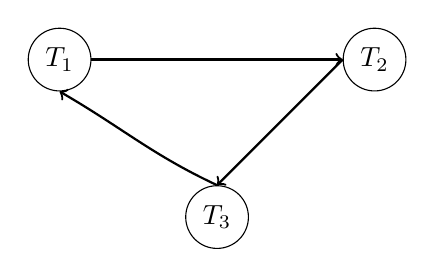
\begin{tikzpicture}
			[task/.style={circle, draw},] 
          	\node[task] (T1) at (0.0, 2.0) {$T_1$}; 
          	\node[task] (T2) at (4.0, 2.0) {$T_2$}; 
          	\node[task] (T3) at (2.0, 0) {$T_3$}; 
           
            \draw[->, thick, draw] (T1.east) to [out=0,in=180] (T2.west); 
            \draw[->, thick, draw] (T2.west) to [out=225,in=45] (T3.north); 
            \draw[->, thick, draw] (T3.north) to [out=155,in=330] (T1.south);
			\end{tikzpicture} 

			\caption{Precedence graph for schedule 1} 
			\label{fig:trans-schedule-1} 
		\end{figure}

		\begin{figure}[H]
			\centering
			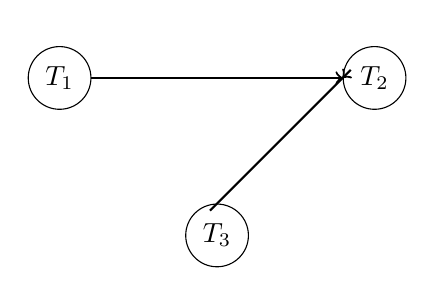
\begin{tikzpicture}
			[task/.style={circle, draw},] 
          	\node[task] (T1) at (0.0, 2.0) {$T_1$}; 
          	\node[task] (T2) at (4.0, 2.0) {$T_2$}; 
          	\node[task] (T3) at (2.0, 0) {$T_3$};  
         	\draw[->, thick, draw] (T1.east) to [out=0,in=180] (T2.west); 
            \draw[->, thick, draw] (T3.north)to [out=225,in=45] (T2.west); 
			\end{tikzpicture} 

			\caption{Precedence graph for schedule 2} 
			\label{fig:trans-schedule-1} 
		\end{figure}		
		
	\item
  \textbf{Schedule 1} couldn't have been generated by a scheduler using
  strict two-phase locking, because $T_1$ takes a read-lock on $X$ and does not
  release it before $T_2$ wants to take a write-lock on $X$. Therefore, under strict 2PL
  it would have to wait for $T_1$ to release its locks.
	
  \textbf{Schedule 2} could have been generated by a scheduler using strict
  two-phase locking (strict 2PL), because at no point does a thread request a
  lock on an already locked resource. The schedule with explicit lock-taking
  looks like this:

  \begin{verbatim}
T1: S(X) R(X)                         X(Y) W(Y) C
T2:                        S(Z) R(Z)              S(X) W(X) X(Y) W(Y) C
T3:           X(Z) W(Z) C
  \end{verbatim}

  Keep in mind that \verb|C| releases all locks held by the thread.
\end{enumerate}

\section{Question 2}

We recall the three validation conditions from the text:
\begin{enumerate}
  \item
    $T_i$ completes (all three phases) before $T_j$ begins.
  \item
    $T_i$ completes before $T_j$ starts its Write phase, and $T_i$ does not
    write any database object read by $T_j$
  \item
    $T_i$ completes its Read phase before $T_j$ completes its Read phase, and
    $T_i$ does not write any database object that is either read or written by
    $T_j$
\end{enumerate}


So for each of the different scenarios we have:
\begin{enumerate}
		\item
		T3 must be rolled back. T1 passes the first condition, but for T2:
			\begin{itemize}
				\item
				Condition 1 fails, because T2 does not complete before T3 starts.
				\item
				Condition 2 fails, because T2 completes before T3 begins with its write phase, but the 
				WriteSet(T2) $\cap$ ReadSet(T3) is not empty, and the offending object is 4.
				\item
				Condition 3 fails, none of the conditions are met.
			\end{itemize}
		
		\item
		T3 must be rolled back. For T1:
			\begin{itemize}
				\item
				Condition 1 fails, because T1 does not complete before T3 begins.
				\item
				Condition 2 fails. T1 does complete before T3 begins with its write phase, but the 
				WriteSet(T1) $\cap$ ReadSet(T3) is not empty, the offending object is 3.
				\item
				Condition 3 fails, because T1 doesn't meet the initial condition.
			\end{itemize}				
		
		\item
		T3 is allowed to commit and condition 2 is necessary to reach the conclusion. T1 completes before T3 
		begins with its write phase, and the WriteSet(T1) $\cap$ ReadSet(T3) is empty. T2 completes 
		before T3 begins with its write phase, and the WriteSet(T2) $\cap$ ReadSet(T3) is empty.			
	
\end{enumerate}
 
\section{Question 3}
\begin{enumerate}
	\item
		\begin{itemize}
		 \item[a)]
       On \textit{SingleLockConcurrentCertainBookStore} we take a global lock at
       the start of our function calls, thus at top level we achieve
       correct before-or-after atomicity.

       For \textit{TwoLevelLockingConcurrentCertainBookStore}, at top-level the
       \textbf{takeGlobalLock} is acquired on exclusive mode when we perform
       \textbf{addBooks} and \textbf{removeBooks}. \textbf{globalReadLock} is
       taken whenever a local lock is taken. This ensures that a global exclusive
       lock can't be taken before all local locks are released.

       At the bottom level, there is one read-write lock for each book in the
       bookstore. We use \textbf{takeLocalWriteLock} on data items that are modified and
       \textbf{takeLocalReadLock} on data items that are only read.
       We do this during the execution of the transaction as needed.
       We release locks on objects at the end of the transaction or in case of some
       exception being thrown.

       At each level the transactions are executed as if in serial order, so the
       \textit{TwoLevelLockingConcurrentCertainBookStore} has the correct
       before-or-after atomicity.
		
		\item[b)]
      We have used two general strategies for testing the concurrency code. The
      first strategy is to have two different threads doing opposite operations.
      At the end, we test that the environment is unchanged. This can for
      example be seen in \verb|testBuyAndAddConcurrent| and
      \verb|testUpdateEditorPicks|.

      The other strategy we use is to have some number of threads repeatedly
      doing an action and a testing thread repeatedly reads the updates and
      checks consistency. This is to ensure that threads can only observe legal
      states. Such tests are for example \verb|testBuyAndAddConsistency|,
      \verb|testRatedBooks| and \verb|testUpdateEditorPicks|. The latter of the
      two uses two threads doing updates and one checking consistency.

		\item[c)]
      We don't have to consider different testing. Because the scheme in
      \textit{SingleLockConcurrentCertainBookStore} is the same as the scheme in
      \textit{TwoLevelLockingConcurrentCertainBookStore}
      
      The use of different strategies would not be a violation of modularity,
      but it might be helpful to still consider it. Different implementations
      have different edge cases where there might be bugs. Taking this into
      consideration when writing tests is a good idea.
		\end{itemize}
  \item
     The \textit{SingleLockConcurrentCertainBookStore} implementation is
     not only equivalent with strict 2PL, it is also equivalent with
     conservative 2PL. This is because all functions immediately take all locks
     (the only lock) they need and release it at the very end of the call.\\

     For \textit{TwoLevelLockingConcurrentCertainBookStore}, things are a little
     more complicated. In 2PL, there is a growing phase and a shrinking
     phase. Locks are taken in the growing phase and released in the shrinking
     phase. Strict 2PL also requires that all exclusive locks are released at
     the very end of the transaction, when either commiting or aborting.

     The growing phase is encoded in our implementation simply as part of the
     function body. The thread acquires locks on objects as it needs them. The
     shrinking is embedded in the \verb|finally| blocks that wrap the function
     body. Here, all locks taken by the transaction are released. Since this
     includes all exclusive locks, the implementation is strict.

     Since we implement a shrinking and growing phase and all exclusive locks
     are released only upon commit or abort, our implementation is equivalent to
     strict 2PL.
	\item
		\begin{itemize}
		 \item
     For \textit{SingleLockConcurrentCertainBookStore}, our locking protocol
     will not lead to deadlocks. We first take \textbf{writeLock} on data items
     that are modified and take \textbf{readLock} on data items that are read,
     then execute transaction, finally release all locks. Therefore there is no
     deadlocks.
		 
		 \item
     For \textit{TwoLevelLockingConcurrentCertainBookStore}, our locking
     protocol will lead to deadlocks. At top-level the \textbf{takeGlobalLock}
     is acquired on exclusive mode when we perform \textbf{addBooks} and
     \textbf{removeBooks}, \textbf{globalReadLock} is in all the other
     operations. At the bottom level, there is one read-write lock for each book
     in the bookstore.

     \textbf{takeLocalWriteLock} on data items that are modified and
     \textbf{takeLocalReadLock} on data items that are read, but do this during
     execution of transaction (as needed). Release locks on objects no longer
     needed during execution of transaction. Therefore we need to know when to 
		 release locks, which may leads to deadlocks.
		\end{itemize}
  \item
    We have no thrashing handling in the implementation, so a large amount of
    requests could simply bog down our store in overhead computations. This is
    especially true for \textit{SingleLockConcurrentCertainBookStore} because of
    the low amount of concurrency in the implementation.
	
  \item
    The concurrency for \textit{SingleLockConcurrentCertainBookStore} is limited
    by the number of operations that modify state, since these need exclusive
    locks and put everything else on hold. In a bookstore, we can expect there
    to be less requests for writing than reading. Since the overhead is pretty
    small, this tradeoff is probably good.\\

    With the two-level locking scheme we get to pay quite a bit more overhead
    than with the single-lock: Our locks live in a map and take $O(n)$ time to
    find every time we need one. If our bookstore has an enormous amount of
    books and a large amount of requests, this might actually have impact on
    performance.

    On the other hand, we achieve the benefit that a write operation no longer
    locks the rest of the bookstore from functioning, which is an advantage if
    the number of requests is large.

\end{enumerate}

\end{document}
